% CAISc 2026 submission: esmc.cpp
% Open-Ended Track. Built on the official caisc_2026 template/style file.
%
% NOTE: This paper requires the conference style file `caisc_2026.sty`
% (obtainable from https://caisc2026.github.io/cfp.html) to be present in the
% same directory. Compile with pdflatex. The default (no-option) mode below
% produces the anonymized submission version with line numbers.

\documentclass{article}

% ready for submission (anonymized, line numbers)
\usepackage{caisc_2026}

\usepackage[utf8]{inputenc} % allow utf-8 input
\usepackage[T1]{fontenc}    % use 8-bit T1 fonts
\usepackage{hyperref}       % hyperlinks
\usepackage{url}            % simple URL typesetting
\usepackage{booktabs}       % professional-quality tables
\usepackage{amsfonts}       % blackboard math symbols
\usepackage{nicefrac}       % compact symbols for 1/2, etc.
\usepackage{microtype}      % microtypography
\usepackage{xcolor}         % colors
\usepackage{graphicx}       % figures
\usepackage{amsmath}        % aligned display math

% Artifact links contain identifying usernames and would break double-blind
% anonymity. Keep this false for the anonymized submission build; set it to true
% for the non-anonymized preprint/camera-ready build (alongside the
% \usepackage[preprint]{caisc_2026} or [final] option) to reveal the URLs.
\newif\ifshowartifacts
\showartifactstrue

\title{esmc.cpp: A Zero-Dependency, Metal-Accelerated C/C++ Runtime for ESM Cambrian Protein Embeddings}

% Anonymized submission: author block is hidden by the style file in the
% default mode. A placeholder is kept here per template instructions.
\author{%
  Anonymous Author(s)\\
  Affiliation withheld for double-blind review\\
  \texttt{anonymous@example.org}\\
}

\begin{document}

\maketitle

\begin{abstract}
Protein language models (PLMs) such as ESM Cambrian (ESM-C) produce per-residue embeddings that power variant-effect prediction, function annotation, and structure-adjacent tasks, but their reference implementations require a heavyweight Python and deep-learning stack that is awkward for edge, batch, and embedded deployment. We port ESM-C 300M, an encoder-only PLM, to \texttt{esmc.cpp}: a standalone C/C++ inference runtime built directly on the ggml/llama.cpp compute substrate, with no Python dependency at inference time. We contribute (i) a GGUF weight schema and converter that maps the native checkpoint layout (fused QKV, fused SwiGLU, no biases, RoPE-NeoX, query/key LayerNorm, residual scaling) to ggml graph operations; (ii) a staged, bottom-up validation pipeline (tokenizer $\to$ layer-0 attention probes $\to$ full-forward cosine similarity) that is engineered to catch the silent numerical failures characteristic of PLM ports; and (iii) a benchmark study on a 16\,GB Apple M1. The F16 runtime reproduces PyTorch embeddings to a mean per-residue cosine of $0.99999$ across 100 Swiss-Prot sequences, and 8-bit quantization preserves $0.99971$ while halving the model file. On Apple Silicon, Metal 4-bit inference reaches $1.2$--$1.4\times$ PyTorch CPU throughput on short and medium sequences at $\sim$520\,MiB peak resident memory and $\sim$228\,MiB on disk, and all 36 tested model/precision/backend/length configurations fit comfortably within the 16\,GB budget. We also document concrete silent-failure case studies, including a single-token vocabulary transposition that corrupted embeddings only for sequences containing asparagine or glutamine.
\end{abstract}

\section{Introduction}
\label{sec:intro}

Protein language models trained with masked language modeling over hundreds of millions to billions of clustered sequences have become a default featurizer for computational biology. ESM Cambrian (ESM-C)~[1] is a recent encoder-only family (300M, 600M, 6B parameters) whose single forward pass yields per-residue embeddings with no autoregressive loop and no growing key/value cache. The official runtime, however, is a PyTorch stack: deploying it on a laptop, an offline batch node, or an embedded system means shipping Python, PyTorch, and a constellation of CUDA/Metal dependencies, which is at odds with reproducibility, cold-start latency, and resource-constrained inference.

The llama.cpp project and its ggml tensor library~[6] have demonstrated that decoder-only language models can be run efficiently as a single self-contained binary with on-disk quantization via the GGUF format~[7]. We ask whether the same engineering discipline transfers to a \emph{bidirectional, encoder-only} protein model, and at what cost to numerical fidelity. This is not a mechanical exercise: ESM-C differs from the widely ported ESM2 family~[2] in several details (SwiGLU instead of GELU, no biases anywhere, RoPE-only positions, a wider context, and a non-standard feed-forward width), and any one of these, if mis-implemented, produces embeddings that are numerically plausible but biologically wrong without raising an error.

This paper makes the following contributions:
\begin{itemize}
  \item \textbf{A systems port.} \texttt{esmc.cpp}, a dependency-minimal C/C++ runtime and C library for ESM-C 300M embeddings on the ggml/llama.cpp stack, with CPU and Apple Metal backends and a small command-line tool (\texttt{esmc-embed}).
  \item \textbf{A GGUF schema and converter} for ESM-C that ingests the native checkpoint layout, splitting fused QKV and fused SwiGLU projections, and that records the empirically measured feed-forward width rather than a formula (Section~\ref{sec:design}).
  \item \textbf{A staged validation methodology} that catches silent numerical failures, together with a set of real bug case studies encountered during the port (Section~\ref{sec:validation}).
  \item \textbf{An empirical study} on consumer Apple Silicon spanning numerical correctness, quantization, throughput, memory footprint, and a downstream ProteinGym variant-effect task (Section~\ref{sec:results}).
\end{itemize}

We deliberately scope the quantitative study to the 300M model on a single 16\,GB M1 host; generalization to 600M and 6B is left as future work (Section~\ref{sec:limitations}).

\section{Background and Related Work}
\label{sec:background}

\paragraph{ESM-C versus ESM2.}
ESM-C is an encoder-only transformer with pre-LayerNorm~[5] blocks, rotary position embeddings (RoPE)~[3], and a gated SwiGLU~[4] feed-forward network. Relative to ESM2~[2], the architectural deltas that govern correctness are summarized in Table~\ref{tab:esm2-vs-esmc}. The most consequential are the replacement of the GELU two-matrix FFN with a three-matrix SwiGLU FFN, the complete absence of biases, RoPE-only positional encoding in the NeoX rotation style, and a feed-forward width of approximately $\nicefrac{8}{3}\,d_{\text{model}}$ rather than $4\,d_{\text{model}}$.

\begin{table}
  \caption{Architectural deltas between ESM2 and ESM-C that determine port correctness.}
  \label{tab:esm2-vs-esmc}
  \centering
  \begin{tabular}{lll}
    \toprule
    Feature & ESM2 & ESM-C \\
    \midrule
    FFN & GELU, 2 matrices & SwiGLU, 3 matrices \\
    Biases & present & none (except pre-QKV LayerNorm bias) \\
    Pre-encoder LayerNorm & yes & no \\
    Positional encoding & learned + RoPE & RoPE only (NeoX) \\
    FFN width & $4\,d_{\text{model}}$ & ${\sim}\nicefrac{8}{3}\,d_{\text{model}}$ (2560 for 300M) \\
    Context length & 1024 & 2048 \\
    \bottomrule
  \end{tabular}
\end{table}

\paragraph{ggml, llama.cpp, and GGUF.}
ggml is a C tensor library with CPU and accelerator backends (including Apple Metal); llama.cpp is the inference infrastructure layered on top of it~[6]. GGUF~[7] is a single-file binary format that stores both model metadata (as typed key/value pairs) and tensors, optionally quantized. We reuse this substrate: our converter emits GGUF, our loader reads it, and our quantizer reuses ggml's block-quantization kernels. The novelty is the ESM-C-specific schema, the encoder forward graph, and the validation harness, not the underlying tensor library.

\paragraph{Quantization.}
We use ggml's $k$-quant and legacy block-quant schemes (Q8\_0, Q4\_K\_M, Q4\_K\_S). A practical constraint surfaces immediately: $k$-quant blocks require the per-row dimension to be a multiple of 256. For ESM-C 300M, $d_{\text{model}}=960$ is not, so only the feed-forward down-projection ($2560$ wide) is $k$-quant-eligible; the remaining per-layer matrices fall back to legacy 32-element blocks (Section~\ref{sec:design}).

\section{System Design}
\label{sec:design}

\subsection{Architecture Fidelity}

ESM-C 300M has 30 layers, $d_{\text{model}}=960$, 15 heads (head dimension 64), a SwiGLU intermediate width of 2560, a context length of 2048, a 33-token vocabulary, LayerNorm $\varepsilon=10^{-5}$, and RoPE $\theta=10000$. The reference forward pass we reproduce is:
\begin{enumerate}
  \item token embedding lookup (no positional embedding table; RoPE handles positions);
  \item for each layer: pre-LayerNorm; separate $Q,K,V$ projections; per-projection query/key LayerNorm; scaling of $Q$ by $1/\sqrt{d_{\text{head}}}$ \emph{before} RoPE; RoPE-NeoX on $Q$ and $K$; bidirectional (non-causal) attention $\operatorname{softmax}(QK^\top)V$; output projection; residual add divided by a residual scale $\sqrt{30/36}\approx0.9129$; then pre-LayerNorm, SwiGLU FFN $W_{\text{down}}(\operatorname{SiLU}(W_{\text{gate}}x)\odot W_{\text{up}}x)$, and a second scaled residual;
  \item a single final LayerNorm producing the per-residue embedding $[\,n_{\text{embd}}\times n_{\text{tokens}}\,]$.
\end{enumerate}
There is no pre-encoder or wrap-around LayerNorm, and no token dropout, both of which were present in ESM2.

\subsection{GGUF Conversion}

The native 300M checkpoint stores fused projections under \texttt{esmc.*} keys rather than the HuggingFace \texttt{model.layers.*} layout. Our converter (i) splits the fused QKV weight into \texttt{attn\_q/k/v}, (ii) splits the fused SwiGLU \texttt{fc1\_weight} into \texttt{ffn\_gate} and \texttt{ffn\_up}, (iii) preserves the pre-QKV LayerNorm weight \emph{and bias} and the per-projection query/key LayerNorm weights, and (iv) reads the feed-forward width directly from the tensor shape and writes it to the GGUF metadata key \texttt{esmc.feed\_forward\_length} (2560) instead of computing it from a formula. LayerNorm weights are stored in F32 regardless of the quantization target. The 300M model maps to 363 tensors (3 global plus 9 per layer $\times$ 30). The full architecture is recorded as GGUF metadata (\texttt{esmc.block\_count}, \texttt{esmc.embedding\_length}, \texttt{esmc.attention.head\_count}, \texttt{esmc.rope.freq\_base}, etc.) so that the C++ loader is data-driven.

\subsection{Inference Graph and Tokenizer}

The forward pass is expressed as a ggml computation graph (token embedding via \texttt{ggml\_get\_rows}; LayerNorm as \texttt{ggml\_norm} followed by an elementwise scale, since there is no additive bias on most norms; RoPE via \texttt{ggml\_rope\_ext} in NeoX mode; non-causal attention with no mask), which ggml dispatches to the CPU or Metal backend. The tokenizer is a direct character-to-index lookup over the fixed 33-token amino-acid alphabet (no subword splitting), prepending \texttt{<cls>} and appending \texttt{<eos>}. The index order is not alphabetical: in particular glutamine (Q) precedes asparagine (N), a detail that caused a silent bug (Section~\ref{sec:validation}).

\subsection{Quantization}

We provide a ggml-only quantizer, \texttt{esmc-quantize}, that calls \texttt{ggml\_quantize\_chunk} directly, bypassing llama.cpp's architecture registry (which does not recognize \texttt{general.architecture = "esmc"}). Because $d_{\text{model}}=960$ is not a multiple of 256, only \texttt{ffn\_down} ($n_{\text{per\_row}}=2560$) uses true $k$-quant blocks; the other five weight matrices per layer use legacy fallbacks. After an initial attempt with Q4\_0 fallbacks produced aggregate cosine of only $0.978$--$0.985$, we raised the fallbacks to Q5\_0/Q8\_0, which restored quality above the $0.995$ target (Section~\ref{sec:results}). Embedding and output tables are kept in F16. The resulting file sizes are listed in Table~\ref{tab:correctness}.

\section{Validation Methodology}
\label{sec:validation}

Because PLM ports fail silently, we validate bottom-up rather than by a single end-to-end check:
\[
\text{M4: token IDs} \;\to\; \text{M5: layer-0 } Q/K \text{ L2 norms} \;\to\; \text{M6: full 30-layer per-residue cosine}.
\]
The pass thresholds are: exact token-ID match against the official tokenizer; relative L2 error $\le 5\%$ for $Q$ and $K$ after layer 0 (post-scale, post-RoPE); per-residue mean cosine $>0.999$ and minimum cosine $>0.99$ against a PyTorch reference (with \texttt{<cls>}/\texttt{<eos>} stripped); and mean-pooled relative L2 error $<1\%$. All outputs are additionally checked for finiteness. The reference is a NumPy/PyTorch reimplementation of the native checkpoint layout, validated independently of the HuggingFace \texttt{transformers} path.

\paragraph{Silent-failure case studies.}
Four bugs found during the port double as cautionary case studies (Table~\ref{tab:bugs}). The most instructive is BUG-002: a transposition of the Q and N tokens in the converter metadata corrupted embeddings only for sequences containing asparagine or glutamine. A short test sequence without N or Q passed validation, while medium and long sequences silently dropped to $\sim$0.95 cosine. This is direct evidence that test sequences must exercise the full token alphabet and that a single short smoke sequence is insufficient.

\begin{table}
  \caption{Silent-failure bugs encountered during the port. Each produced wrong embeddings without an error.}
  \label{tab:bugs}
  \centering
  \begin{tabular}{lll}
    \toprule
    Bug & Root cause & Effect (after fix) \\
    \midrule
    BUG-001 & \texttt{.npy} header omitted trailing newline byte & NaN output $\to$ valid floats \\
    BUG-002 & Q/N tokens swapped (indices 16/17) & medium cosine $0.953 \to 0.99999$ \\
    BUG-003 & $Q$ scaled at softmax instead of before RoPE & $Q$ norm error $700\% \to 0.0025\%$ \\
    BUG-004 & \texttt{nan <= 0.999} is False in Python (false PASS) & added explicit finiteness checks \\
    \bottomrule
  \end{tabular}
\end{table}

\section{Experiments and Results}
\label{sec:results}

All experiments run on an Apple M1 (arm64, 16\,GB unified memory, macOS 26.5). The reference is the official PyTorch ESM-C 300M loaded from the native checkpoint. Numerical correctness uses 100 reviewed human Swiss-Prot~[9] sequences bucketed by length (34 small, 33 medium, 33 large); throughput and memory use a fixed length-bucketed FASTA (short 47, medium 235, long 850 tokens including \texttt{<cls>}/\texttt{<eos>}). Each result corresponds to a single host and a single run; we discuss the absence of error bars in Section~\ref{sec:limitations}.

\subsection{Numerical Correctness and Quantization}

Table~\ref{tab:correctness} reports per-residue agreement with the PyTorch reference across precisions. F16 reproduces the reference to a mean cosine of $0.99999$ on all 100 sequences, and a separate F32 build is numerically near-identical to the reference (mean cosine $1.000000$, mean-pool L2 $\sim10^{-6}$), establishing the upper bound on agreement and confirming that the residual F16 gap is rounding, not an architectural error. The CPU and Metal backends agree with each other to mean cosine $>0.9999$, so the Metal path introduces no additional error.

\begin{table}
  \caption{Numerical fidelity and size by precision (300M, 100 Swiss-Prot sequences, CPU). Pass = per-sequence mean cosine $>0.999$ (F16/Q8\_0) or $>0.995$ (Q4\_K\_*). File size relative to F16 (634\,MiB) in parentheses.}
  \label{tab:correctness}
  \centering
  \begin{tabular}{lccccc}
    \toprule
    Precision & Aggregate mean cosine & Pass rate & Worst min cosine & Max mean-pool L2 & File size \\
    \midrule
    F16    & 0.999985 & 100/100 & 0.999711 & 0.0030 & 634\,MiB (1.00) \\
    Q8\_0   & 0.999714 & 100/100 & 0.994269 & 0.0164 & 337\,MiB (0.53) \\
    Q4\_K\_M & 0.995966 & 91/100  & 0.940125 & 0.0656 & 237\,MiB (0.37) \\
    Q4\_K\_S & 0.995228 & 75/100  & 0.928064 & 0.0709 & 228\,MiB (0.36) \\
    \bottomrule
  \end{tabular}
\end{table}

Q8\_0 is a safe default: it passes the strict per-sequence threshold on all 100 sequences at $0.53\times$ the F16 size. Both 4-bit schemes pass the aggregate $0.995$ target, but not on every individual sequence, and failures concentrate in short sequences (for Q4\_K\_M, 9 of 9 failures are in the small bucket). This is consistent with quantization error being a roughly fixed absolute perturbation that matters more when there are fewer residues to average over. Q4\_K\_M dominates Q4\_K\_S (91 versus 75 passes) and is the recommended 4-bit choice for this architecture.

\subsection{Throughput}

Figure~\ref{fig:throughput} and Table~\ref{tab:throughput} summarize single-sequence throughput; PyTorch CPU/MPS baselines and each \texttt{esmc.cpp} configuration are run in separate processes so resident models do not interfere. The best \texttt{esmc.cpp} configuration beats PyTorch CPU on short ($1.41\times$, Metal Q4\_K\_S) and medium ($1.23\times$, Metal Q4\_K\_M) sequences while using roughly $3\times$ less model memory, but PyTorch MPS remains the fastest backend on this hardware, and on long sequences \texttt{esmc.cpp} reaches only $0.76\times$ PyTorch CPU. The CPU path is not competitive at any precision, and 4-bit quantization actually \emph{reduces} CPU throughput (Q4\_K\_M medium is $0.50\times$ F16 CPU) because dequantization overhead exceeds the bandwidth savings without repacked layouts; on Metal, by contrast, quantization helps and the Metal-over-CPU speedup at medium length reaches $2.86\times$ (F16) to $6.70\times$ (Q4\_K\_M). The long-sequence collapse is the signature of naive $O(n^2)$ attention and per-forward graph overhead, which we have begun to address in a separate performance roadmap.

\begin{figure}
  \centering
  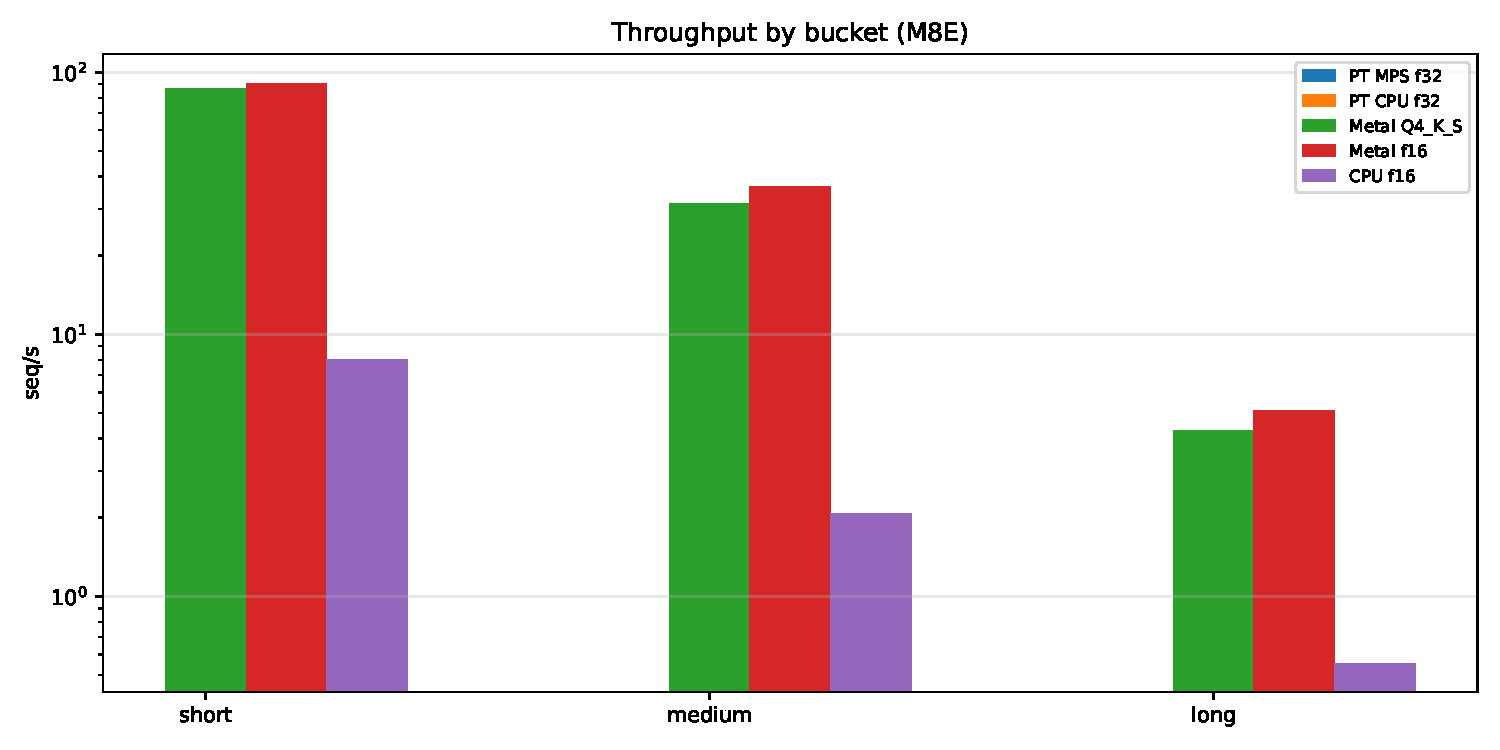
\includegraphics[width=0.85\linewidth]{figures/throughput_seqps.pdf}
  \caption{Single-sequence throughput (seq/s) by length bucket for the best \texttt{esmc.cpp} Metal configurations against PyTorch CPU and MPS baselines. Higher is better.}
  \label{fig:throughput}
\end{figure}

\begin{table}
  \caption{Throughput (seq/s) for representative configurations, with the medium-bucket ratio against PyTorch CPU and the long-bucket peak resident memory.}
  \label{tab:throughput}
  \centering
  \begin{tabular}{llccccc}
    \toprule
    Configuration & Backend & short & medium & long & vs PT CPU (med) & Peak RSS (long) \\
    \midrule
    PyTorch f32 & MPS    & 29.29 & 10.11 & 2.83 & $2.22\times$ & 282\,MiB \\
    PyTorch f32 & CPU    & 10.31 & 4.56  & 1.74 & $1.00\times$ & 1588\,MiB \\
    \texttt{esmc.cpp} Q4\_K\_S & Metal & 14.54 & 5.56 & 1.33 & $1.22\times$ & 519\,MiB \\
    \texttt{esmc.cpp} Q4\_K\_M & Metal & 14.34 & 5.62 & 1.33 & $1.23\times$ & 531\,MiB \\
    \texttt{esmc.cpp} Q8\_0   & Metal & 12.53 & 5.50 & 1.33 & $1.21\times$ & 736\,MiB \\
    \texttt{esmc.cpp} F16    & Metal & 8.61  & 4.80 & 1.29 & $1.05\times$ & 1323\,MiB \\
    \texttt{esmc.cpp} F16    & CPU   & 5.83  & 1.68 & 0.33 & $0.37\times$ & 7426\,MiB \\
    \texttt{esmc.cpp} Q4\_K\_M & CPU   & 3.85  & 0.84 & 0.18 & $0.18\times$ & 6632\,MiB \\
    \bottomrule
  \end{tabular}
\end{table}

\subsection{Memory Footprint}

Figure~\ref{fig:memory} shows long-bucket peak resident set size (RSS) across all 36 configurations measured with \texttt{/usr/bin/time -l} in fresh processes. Every configuration fits within the 16\,GB budget; the worst case (CPU F16, long) peaks at 7426\,MiB, or 45.3\% of the machine. The Metal path is the memory sweet spot: Metal Q4\_K\_S peaks at $\sim$519\,MiB and, importantly, its peak is essentially flat across sequence length ($+9$\,MiB from short to long), whereas CPU peak RSS scales $1.7\times$ (F32) to $9.4\times$ (Q4\_K\_S) from short to long. CPU peak memory is dominated by per-forward graph and attention scratch, not weight bytes: CPU F16 long (7426\,MiB) exceeds CPU F32 long (3989\,MiB) despite holding half the model bytes, and quantization does not meaningfully reduce CPU peak (Q4 long remains $\sim$6.6\,GiB). We therefore recommend Metal Q4\_K\_M/Q4\_K\_S for deployment: $\sim$520\,MiB peak RAM, $\sim$230\,MiB on disk, and $1.2$--$1.4\times$ PyTorch CPU throughput on short/medium sequences.

\begin{figure}
  \centering
  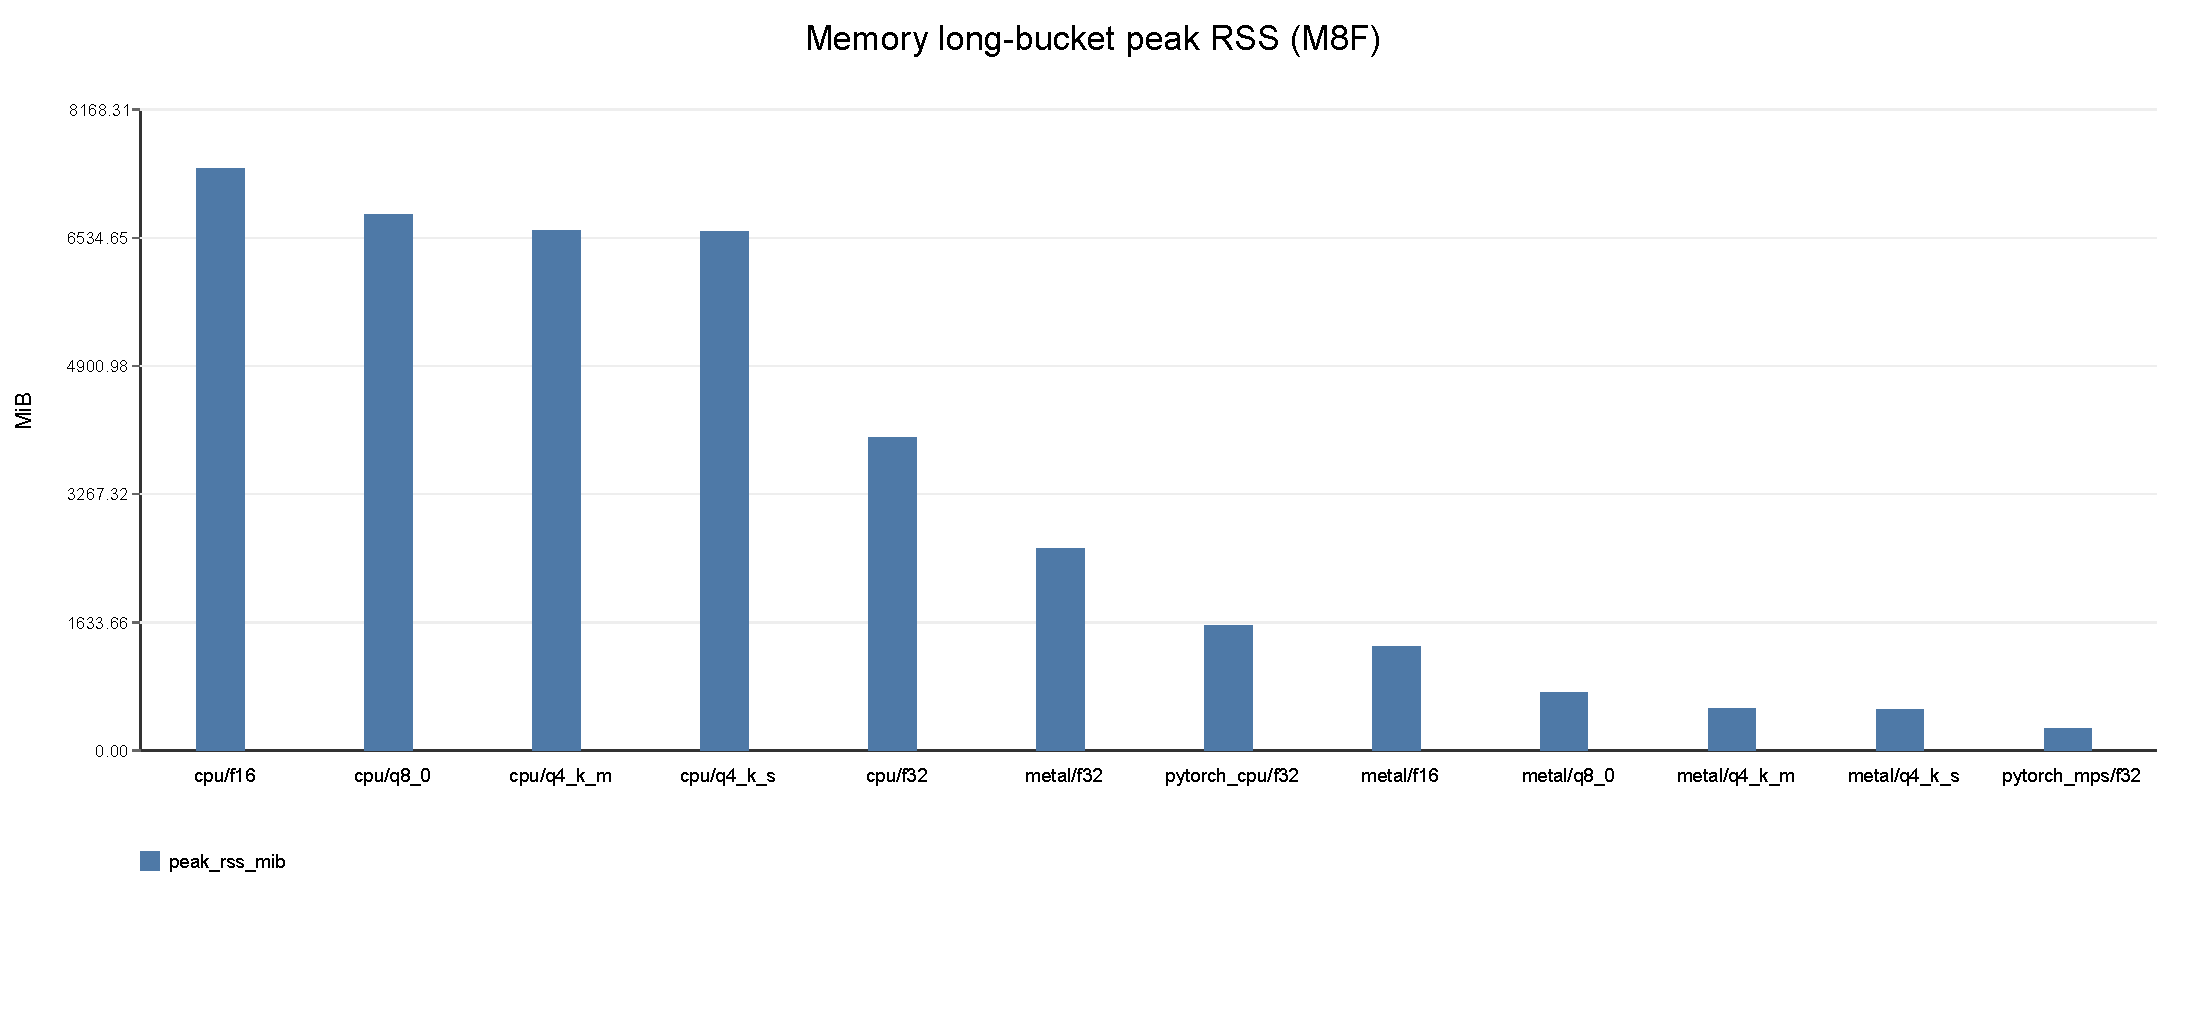
\includegraphics[width=0.85\linewidth]{figures/memory_long_rss.pdf}
  \caption{Long-bucket peak resident set size (MiB) by backend/precision. The CPU configurations dominate the top of the chart; Metal quantized configurations are the lowest. Lower is better.}
  \label{fig:memory}
\end{figure}

\subsection{Downstream Variant-Effect Preservation}

To test that quantization preserves \emph{biological} utility rather than only vector cosine, we ran a ProteinGym~[8] deep-mutational-scanning task over 10 short stability assays~[10] (1000 variants each). We score each variant by the cosine between the mean-pooled embeddings of the mutant and wild-type sequences, and report rank metrics relative to the PyTorch reference; preservation passes when the per-assay metric is within $0.01$ of the reference. Figure~\ref{fig:downstream} and Table~\ref{tab:downstream} show that F16 is effectively identical to the reference (50/50 metric rows pass), Q8\_0 preserves rank correlations well (Spearman/Pearson/Kendall all 10/10, with misses only in stricter top/bottom-decile overlap diagnostics), while the 4-bit schemes are less stable on the Spearman gate (Q4\_K\_M 7/10, Q4\_K\_S 6/10). We emphasize that the absolute Spearman varies widely across assays (reference range $-0.64$ to $0.61$); the embedding-cosine scorer is a preservation probe, not a calibrated zero-shot predictor (Section~\ref{sec:limitations}).

\begin{figure}
  \centering
  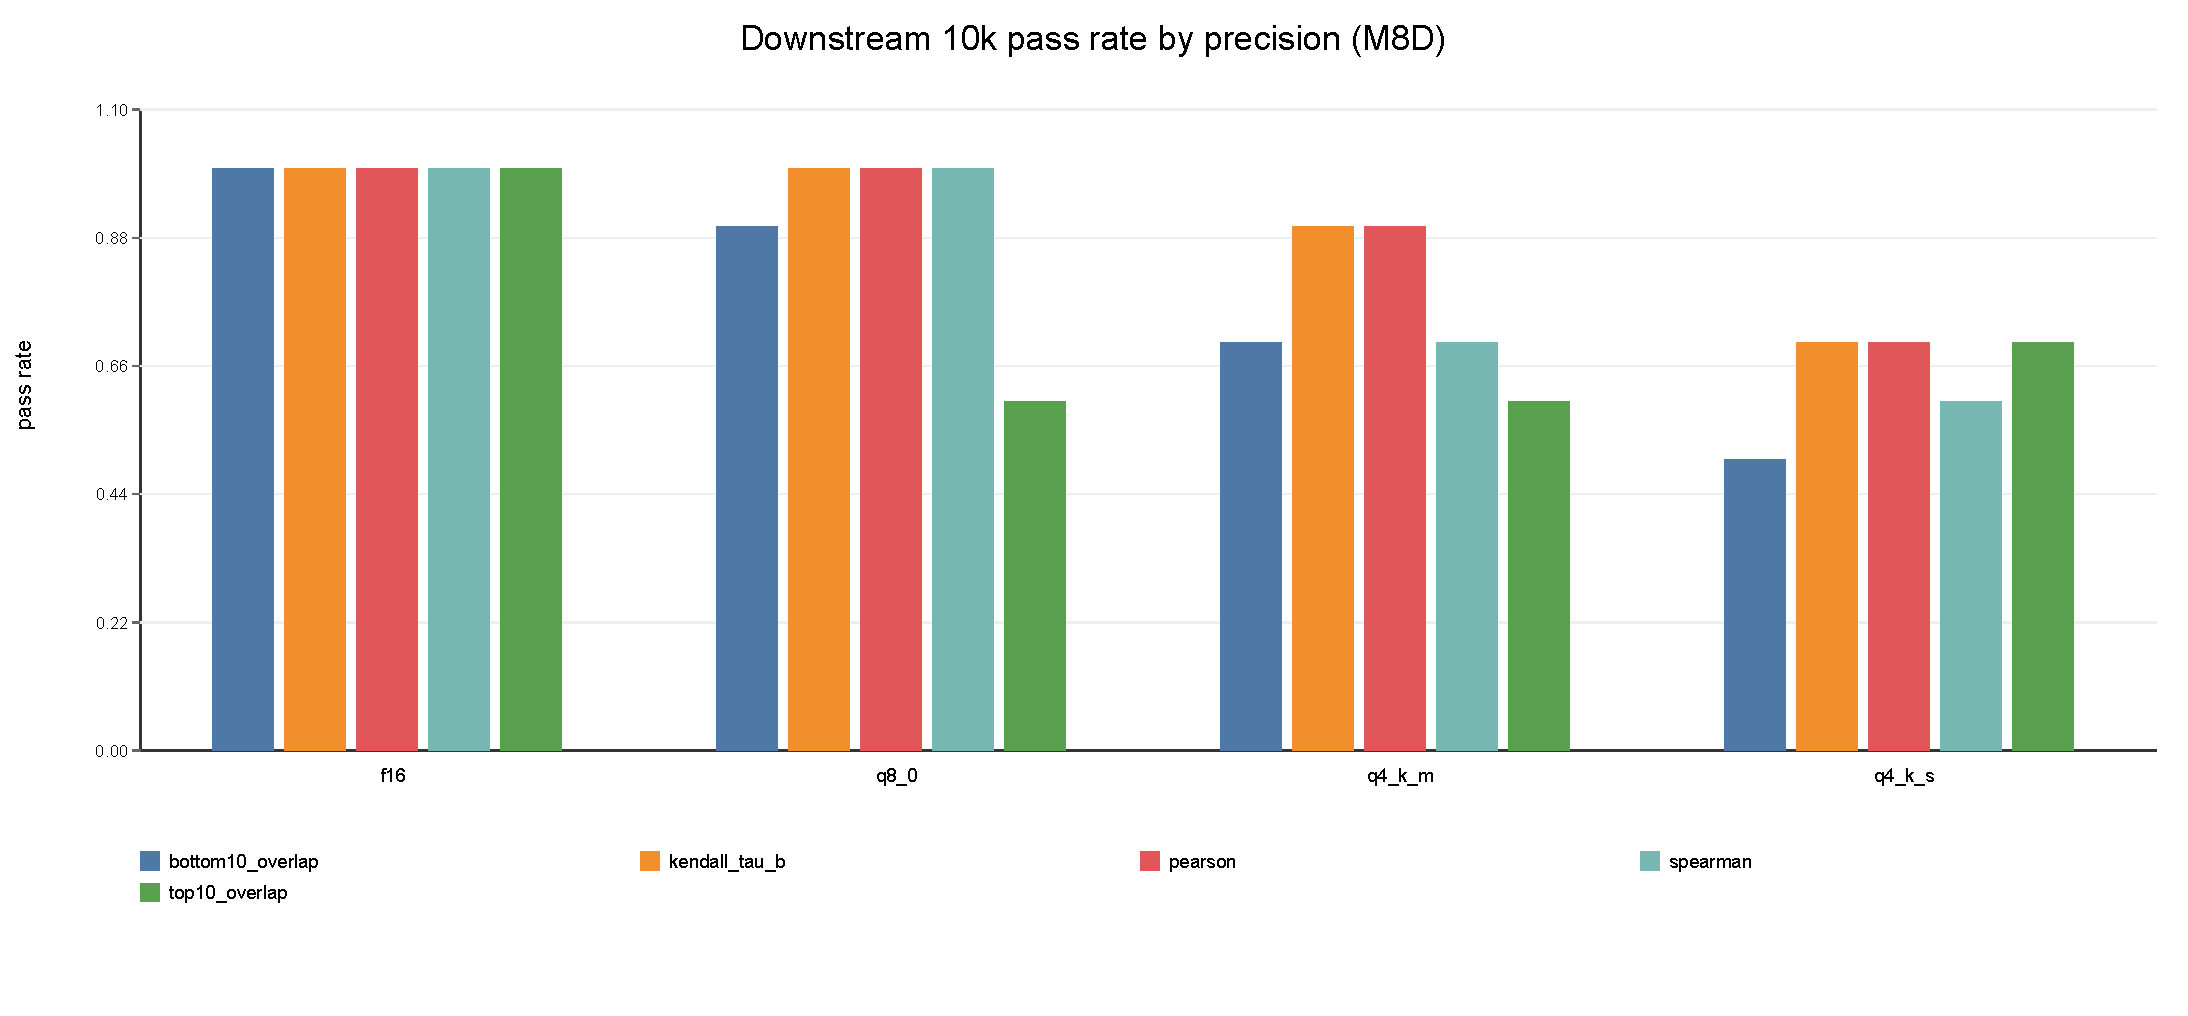
\includegraphics[width=0.85\linewidth]{figures/downstream_10k_pass_rate.pdf}
  \caption{ProteinGym 10-assay downstream preservation pass rates by precision, broken down by metric (Spearman, Pearson, Kendall $\tau_b$, top-/bottom-decile overlap). Pass = within $0.01$ of the PyTorch reference per assay.}
  \label{fig:downstream}
\end{figure}

\begin{table}
  \caption{Downstream preservation versus PyTorch on 10 ProteinGym assays. Pass = $|\Delta|\le0.01$ per assay.}
  \label{tab:downstream}
  \centering
  \begin{tabular}{lccc}
    \toprule
    Precision & All-metric pass & Spearman pass & Mean $|\Delta\,\text{Spearman}|$ \\
    \midrule
    F16    & 50/50 & 10/10 & 0.000585 \\
    Q8\_0   & 45/50 & 10/10 & 0.003104 \\
    Q4\_K\_M & 38/50 & 7/10  & 0.006763 \\
    Q4\_K\_S & 32/50 & 6/10  & 0.011048 \\
    \bottomrule
  \end{tabular}
\end{table}

\section{Discussion and Limitations}
\label{sec:limitations}

\paragraph{Scope.}
The quantitative study covers only the 300M model on a single 16\,GB M1 host. The 600M and 6B variants are not yet ported or benchmarked; in particular, 6B has $d_{\text{model}}=2560$ (a multiple of 256), so we expect $k$-quant to behave qualitatively differently and the memory story to be the binding constraint rather than throughput.

\paragraph{Statistical significance.}
Each correctness, throughput, and memory number is a single run on a single machine; we report run-to-run throughput stability of within $\pm2\%$ from a repeated F16 measurement but do not provide formal error bars or multi-host variance. Headline claims should be read as point estimates on this hardware.

\paragraph{$k$-quant limitation.}
At $d_{\text{model}}=960$, only one of seven weight matrices per layer uses true $k$-quant blocks; the rest use legacy fallbacks. This both caps the achievable compression and explains the short-sequence quality concentration. Claims about 4-bit quality should be qualified by the 75--91\% per-sequence pass rate or restricted to sequences above a minimum length.

\paragraph{Throughput regime.}
\texttt{esmc.cpp} is a portability and memory-efficiency path, not a universal throughput win: it beats PyTorch CPU only on short/medium sequences with Metal quantization, trails PyTorch MPS everywhere, and is bottlenecked on long sequences by naive $O(n^2)$ attention and per-forward overhead. Flash attention and persistent GPU-resident graphs are the obvious next steps.

\paragraph{Downstream proxy.}
The downstream task measures whether quantization \emph{preserves} the PyTorch embedding behavior, using a cosine-based proxy rather than ProteinGym's masked-marginal likelihood. It supports preservation claims for F16 and Q8\_0 rank metrics but does not establish absolute biological prediction quality, and does not support blanket 4-bit preservation claims under the $0.01$ Spearman tolerance.

\section{Conclusion}
\label{sec:conclusion}

We ported ESM-C 300M to \texttt{esmc.cpp}, a dependency-minimal C/C++ runtime on the ggml/llama.cpp stack, with a GGUF schema and converter for the native checkpoint layout and a staged validation pipeline designed to catch silent numerical failures. The F16 runtime reproduces PyTorch embeddings to a mean cosine of $0.99999$, 8-bit quantization preserves $0.99971$ at half the size, and Metal 4-bit inference offers a compelling memory-efficiency profile ($\sim$520\,MiB peak, $\sim$230\,MiB on disk) while matching or beating PyTorch CPU throughput on short and medium sequences. The bug case studies argue that alphabet-covering test sequences and bottom-up numeric probes are necessary, not optional, when porting protein language models. Extending the runtime to 600M and 6B, adding flash attention and GPU-resident graphs, and batching for throughput-bound workloads are the natural next steps.

\begin{ack}
Acknowledgments are omitted in the anonymized submission and will be added to the camera-ready version. The authors declare no funding or competing interests related to this work.
\end{ack}

\section*{References}

\medskip
{
\small

[1] EvolutionaryScale Team (2024) ESM Cambrian: a frontier protein language model. \textit{EvolutionaryScale Technical Blog}. \url{https://www.evolutionaryscale.ai/blog/esm-cambrian}

[2] Lin, Z., Akin, H., Rao, R., Hie, B., Zhu, Z., Lu, W., et al.\ (2023) Evolutionary-scale prediction of atomic-level protein structure with a language model. \textit{Science} \textbf{379}(6637):1123--1130.

[3] Su, J., Lu, Y., Pan, S., Wen, B.\ \& Liu, Y.\ (2021) RoFormer: Enhanced transformer with rotary position embedding. \textit{arXiv:2104.09864}.

[4] Shazeer, N.\ (2020) GLU variants improve transformer. \textit{arXiv:2002.05202}.

[5] Ba, J.L., Kiros, J.R.\ \& Hinton, G.E.\ (2016) Layer normalization. \textit{arXiv:1607.06450}.

[6] Gerganov, G.\ and the llama.cpp contributors (2023--2025) llama.cpp and the ggml tensor library. \url{https://github.com/ggml-org/llama.cpp}

[7] llama.cpp contributors (2023--2025) GGUF: a single-file format for ggml models. \url{https://github.com/ggml-org/ggml/blob/master/docs/gguf.md}

[8] Notin, P., Kollasch, A.W., Ritter, D., van Niekerk, L., Paul, S., Spinner, H., et al.\ (2023) ProteinGym: Large-scale benchmarks for protein fitness prediction and design. In \textit{Advances in Neural Information Processing Systems 36}.

[9] The UniProt Consortium (2023) UniProt: the universal protein knowledgebase in 2023. \textit{Nucleic Acids Research} \textbf{51}(D1):D523--D531.

[10] Tsuboyama, K., Dauparas, J., Chen, J., Laine, E., Mohseni Behbahani, Y., Weinstein, J.J., et al.\ (2023) Mega-scale experimental analysis of protein folding stability in biology and design. \textit{Nature} \textbf{620}(7973):434--444.
}

%%%%%%%%%%%%%%%%%%%%%%%%%%%%%%%%%%%%%%%%%%%%%%%%%%%%%%%%%%%%
\appendix
\section{Reproduction and Tensor Naming}
\label{app:repro}

\paragraph{Code and data availability.}
\ifshowartifacts
The complete runtime, GGUF converter, quantizer, and benchmark harnesses are
open source at \url{https://github.com/AnanyaP-WDW/esmc.cpp}. The pre-converted
GGUF model files (F32/F16/Q8\_0/Q4\_K\_M/Q4\_K\_S), together with a model card
and the benchmark summary, are published at
\url{https://huggingface.co/AnanyaPathak/esmc-300m-gguf}.
\else
The complete runtime, GGUF converter, quantizer, and benchmark harnesses are
released as open source, and the pre-converted GGUF model files are published on
the HuggingFace Hub with a model card and benchmark summary. The repository and
model URLs are withheld here to preserve anonymity and are provided in the
anonymized supplementary material.
\fi

\paragraph{End-to-end reproduction (300M).}
\begin{verbatim}
# Environment + weights (torch is needed for the PyTorch reference/baselines)
python3 -m venv .venv
.venv/bin/pip install -r tools/requirements.txt
.venv/bin/pip install -e ./ggml/gguf-py
.venv/bin/pip install torch
hf download EvolutionaryScale/esmc-300m-2024-12 --local-dir ./esmc-300m

# Build C++ (esmc-embed, esmc-bench, esmc-quantize)
cmake -B build -DCMAKE_BUILD_TYPE=Release && cmake --build build -j8

# Convert (F16 + F32) + verify
.venv/bin/python tools/convert_esmc_to_gguf.py ./esmc-300m \
    ./models/esmc-300m-f16.gguf --dtype f16
.venv/bin/python tools/convert_esmc_to_gguf.py ./esmc-300m \
    ./models/esmc-300m-f32.gguf --dtype f32
.venv/bin/python tools/verify_gguf.py ./models/esmc-300m-f16.gguf

# Staged validation (milestones 4-7)
.venv/bin/python tests/test_tokenizer.py        # tokenizer
.venv/bin/python tests/check_layer0_qk.py       # layer-0 Q/K probe
.venv/bin/python tests/validate.py --no-metal   # full forward (CPU)
.venv/bin/python tests/validate.py --metal --compare-cpu-metal

# Quantize from the F32 GGUF
./build/esmc-quantize models/esmc-300m-f32.gguf models/esmc-300m-Q8_0.gguf   Q8_0
./build/esmc-quantize models/esmc-300m-f32.gguf models/esmc-300m-Q4_K_M.gguf Q4_K_M
./build/esmc-quantize models/esmc-300m-f32.gguf models/esmc-300m-Q4_K_S.gguf Q4_K_S

# Regenerate the 100-sequence PyTorch reference (not shipped; ~107 MB)
.venv/bin/python tests/generate_reference.py \
    --fasta benchmarks/sequences_correctness.fasta \
    --output tests/reference_embeddings.npz

# Benchmarks
.venv/bin/python benchmarks/correctness.py
.venv/bin/python benchmarks/throughput.py --config benchmarks/config_throughput_300m.json
.venv/bin/python benchmarks/memory.py     --config benchmarks/config_memory_300m.json
.venv/bin/python benchmarks/fetch_proteingym_subset.py --download \
    --selection-mode multi-assay --max-assays 10 --max-rows 1000 --min-rows 1000 \
    --max-length 512 --output-dir benchmarks/proteingym_subset_10k \
    --manifest benchmarks/datasets/proteingym_subset_10k_manifest.json
.venv/bin/python benchmarks/downstream.py --config benchmarks/config_downstream_300m_10k.json
\end{verbatim}

\paragraph{Canonical GGUF tensor names.}
Global tensors are \texttt{token\_embd.weight}, \texttt{output\_norm.weight}, and \texttt{output.weight}; per-layer tensors follow the \texttt{blk.\{i\}.*} pattern (\texttt{attn\_q/k/v/output.weight}, \texttt{attn\_norm.weight}/\texttt{.bias}, \texttt{attn\_q\_norm.weight}, \texttt{attn\_k\_norm.weight}, \texttt{ffn\_norm.weight}, \texttt{ffn\_gate/up/down.weight}), for a total of 363 tensors at 300M.

\newpage

\section*{Conference For AI Scientists 2026 - AI Involvement Checklist}
\label{checklist_ai_involvement}

\subsection*{Research Stage Assessment}

\begin{enumerate}

    \item \textbf{Hypothesis development}: Hypothesis development includes the process by which you came to explore this research topic and research question. This can involve the background research performed by either researchers or by AI. This can also involve whether the idea was proposed by researchers or by AI.

    Answer: \involvementB{}

    Iteration Effort: \iterationMedium{}

    Explanation: The high-level idea (port an encoder-only protein language model to the ggml/llama.cpp stack and quantify the fidelity/efficiency trade-off) was framed jointly: humans set the goal and the consumer-hardware framing, while the AI system surveyed the ESM-C architecture, identified the ESM2 vs.\ ESM-C deltas that matter for correctness, and proposed the staged-validation and benchmark structure. Iteration was moderate, spanning several rounds of refining scope (300M-only) and benchmark choices.

    \item \textbf{Experimental design and implementation}: This category includes design of experiments that are used to test the hypotheses, coding and implementation of computational methods, and the execution of these experiments.

    Answer: \involvementC{}

    Iteration Effort: \iterationHigh{}

    Explanation: The AI system authored the large majority of the converter, the C++ ggml forward graph, the quantizer, and the benchmark harnesses, with humans providing direction, running commands on the target hardware, and approving milestone gates. Implementation required extensive trial-and-error (well over 100 substantive attempts), particularly around RoPE style, query scaling order, the fused-projection split, and the $k$-quant fallback policy.

    \item \textbf{Analysis of data and interpretation of results}: This category encompasses any process to organize and process data for the experiments in the paper. It also includes interpretations of the results of the study.

    Answer: \involvementC{}

    Iteration Effort: \iterationMedium{}

    Explanation: The AI system computed the cosine/L2 metrics, aggregated the correctness/throughput/memory/downstream tables, and drafted the interpretations (e.g., the short-sequence quantization concentration and the CPU-vs-Metal throughput split). Humans verified the numbers against raw artifacts and sanity-checked the conclusions.

    \item \textbf{Writing}: This includes any processes for compiling results, methods, etc. into the final paper form. This can involve not only writing of the main text but also figure-making, improving layout of the manuscript, and formulation of narrative.

    Answer: \involvementC{}

    Iteration Effort: \iterationMedium{}

    Explanation: The AI system drafted the full manuscript, tables, and figure captions from the project's lab notebook and result files, and converted the benchmark plots to the embedded figures. Humans guided the structure, enforced the template/format constraints, and reviewed for accuracy.

\end{enumerate}

\subsection*{AI System Documentation}

\begin{enumerate}
    \setcounter{enumi}{4}

    \item \textbf{AI systems used}: Describe all AI systems used in this research without naming specific products or models. Use system-level descriptors only (e.g., ``a frontier large language model'', ``a protein structure prediction system'', ``a custom multi-agent framework built on open-source models''). Include relevant details such as system type, scale, and capabilities. \textbf{Specific model and product names should only be included in the camera-ready version.}

    Description: A frontier large language model operating as an autonomous coding agent inside an integrated development environment, with tool access to the shell, file system, and code search. It was used for architecture research, C/C++ and Python implementation, experiment execution orchestration, data analysis, and manuscript drafting. No separate specialized scientific model was used beyond the ESM-C protein language model that is the subject of the port.

    \item \textbf{Observed AI Limitations}: What specific limitations and failure modes have you observed when using AI as a partner or lead author?

    Description: The dominant failure mode was \emph{silent numerical error}: the agent produced code that ran and yielded plausible embeddings while being subtly wrong (e.g., a transposed vocabulary entry that only affected sequences containing certain amino acids, and an incorrectly ordered query scaling relative to RoPE). These were caught only by the staged, alphabet-covering validation harness, not by the agent's own judgement. The agent also tended toward optimistic claims and required human gating to scope conclusions honestly (e.g., not over-claiming 4-bit quality or single-host throughput), and it occasionally needed correction on platform-specific edge cases such as the $k$-quant block-size constraint at $d_{\text{model}}=960$.

\end{enumerate}

\newpage

\section*{Conference For AI Scientists 2026 - Reproducibility and Responsibility Checklist}
\label{checklist_reproducibility}

\begin{enumerate}

\item {\bf Claims}
    \item[] Question: Do the main claims made in the abstract and introduction accurately reflect the paper's contributions and scope?
    \item[] Answer: \answerYes{}
    \item[] Justification: The abstract and Section~\ref{sec:intro} state the contributions (port, GGUF schema/converter, staged validation, 300M empirical study) and explicitly scope the study to 300M on a single M1 host, matching the results in Section~\ref{sec:results} and the limitations in Section~\ref{sec:limitations}.

\item {\bf Limitations}
    \item[] Question: Does the paper discuss the limitations of the work performed by the authors?
    \item[] Answer: \answerYes{}
    \item[] Justification: Section~\ref{sec:limitations} discusses scope (300M only), absence of error bars, the $k$-quant structural limitation, the non-competitive CPU/long-sequence regime, and the downstream proxy caveat.

\item {\bf Theory assumptions and proofs}
    \item[] Question: For each theoretical result, does the paper provide the full set of assumptions and a complete (and correct) proof?
    \item[] Answer: \answerNA{}
    \item[] Justification: The paper is a systems and empirical study; it contains no theorems or formal proofs.

    \item {\bf Experimental result reproducibility}
    \item[] Question: Does the paper fully disclose all the information needed to reproduce the main experimental results of the paper to the extent that it affects the main claims and/or conclusions of the paper (regardless of whether the code and data are provided or not)?
    \item[] Answer: \answerYes{}
    \item[] Justification: Section~\ref{sec:design}, Section~\ref{sec:validation}, Section~\ref{sec:results}, and Appendix~\ref{app:repro} give the architecture, conversion, quantization mix, validation thresholds, datasets, hardware, and exact reproduction commands.

\item {\bf Open access to data and code}
    \item[] Question: Does the paper provide open access to the data and code, with sufficient instructions to faithfully reproduce the main experimental results, as described in supplemental material?
    \item[] Answer: \answerYes{}
    \item[] Justification: The runtime, converter, quantizer, and benchmark harnesses are released with the project, and the benchmark sequences are derived from public Swiss-Prot and ProteinGym data with provenance manifests; the model weights are publicly available ESM-C 300M checkpoints. \ifshowartifacts Code: \url{https://github.com/AnanyaP-WDW/esmc.cpp}; pre-converted GGUF models and model card: \url{https://huggingface.co/AnanyaPathak/esmc-300m-gguf}. \else (Repository and model URLs anonymized at submission time; provided in the anonymized supplement.)\fi

\item {\bf Experimental setting/details}
    \item[] Question: Does the paper specify all the training and test details (e.g., data splits, hyperparameters, how they were chosen, type of optimizer, etc.) necessary to understand the results?
    \item[] Answer: \answerYes{}
    \item[] Justification: No training is performed (inference port). The model hyperparameters, precisions, sequence buckets, iteration/warmup counts, and pass thresholds are specified in Sections~\ref{sec:design}--\ref{sec:results}.

\item {\bf Experiment statistical significance}
    \item[] Question: Does the paper report error bars suitably and correctly defined or other appropriate information about the statistical significance of the experiments?
    \item[] Answer: \answerNo{}
    \item[] Justification: Results are single runs on a single host; we report run-to-run throughput stability ($\pm2\%$) but do not provide formal error bars, and we flag this explicitly in Section~\ref{sec:limitations}.

\item {\bf Experiments compute resources}
    \item[] Question: For each experiment, does the paper provide sufficient information on the computer resources (type of compute workers, memory, time of execution) needed to reproduce the experiments?
    \item[] Answer: \answerYes{}
    \item[] Justification: All experiments run on an Apple M1 with 16\,GB unified memory (macOS 26.5); peak memory per configuration is reported in Section~\ref{sec:results}, and indicative runtimes (e.g., the downstream run) are noted.

\item {\bf Research Ethics}
    \item[] Question: Does the research conducted in the paper conform with the \href{https://neurips.cc/Conferences/2026/MainTrackHandbook}{NeurIPS Code of Ethics}, except where CAISc's AI authorship policies apply?
    \item[] Answer: \answerYes{}
    \item[] Justification: The work uses public protein sequence data and open model weights, involves no human subjects or personal data, and conforms to the Code of Ethics except for the AI-authorship aspects governed by CAISc policy and documented in the AI Involvement Checklist.

\item {\bf Broader impacts}
    \item[] Question: Does the paper discuss both potential positive societal impacts and negative societal impacts of the work performed?
    \item[] Answer: \answerYes{}
    \item[] Justification: Lowering the deployment cost of protein embeddings broadens access for research and education (positive); as with any protein-modeling tool there is a dual-use consideration, but this work only makes an existing public model cheaper to run rather than increasing its capability, so the marginal risk is limited.

\end{enumerate}

\end{document}
